%----------------------------------------------------------------------------
\chapter{Előismeretek}
%----------------------------------------------------------------------------

%\section{Részleges modellek fajtái}
%\subsection{May}
%\subsection{Abs}
%\subsection{Var}
%\subsection{OW}
\section{Bemutatás egy példa segítségével}
%pl osztálydiagram
A részleges modellezést legegyszerűbben egy gyakorlati példán lehet bemutatni. Vegyük példának az UML objektumdiagramját. Az UML (Unified Modeling Language) egy szabványos, objektumorientált modellezési nyelv, ami a tervezést, fejlesztést és egyéb folyamatokat segíti. Ezt a nyelvet informatikában és egyéb üzleti területeken egyaránt alkalmazzák. Magában foglal több diagram típust is.
Az objektumdiagram egy strukturális diagram, az osztálydiagramnak egy példánya, egy konkrét megvalósítás. Példának vegyük egy jármű objektum diagramját. 

\begin{figure}[!ht]
	\centering
	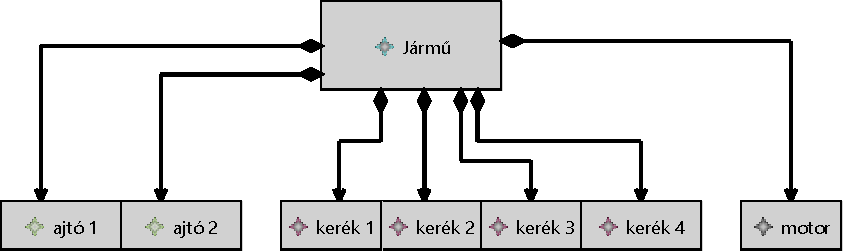
\includegraphics[width=120mm]{figures/vehicle.pdf}
	\caption{Jármű egyszerűsített objektumdiagramja} 
\end{figure}

\section{Metamodell}
A metamodell az tulajdonképpen egy modellnek a modellje. Egy olyan alapséma, amire illeszkedik az összes hozzá tartozó magasabb absztrakciós szinttel rendelkező modell. 
Tegyük fel hogy M* modell M1 modellnek a metamodellje.
Akkor M* metamodell meghatározza az M1 modellben lévő elemeket, attribútumokat és ezeknek lehetséges kapcsolatait. Ilyen metamodell például az objektumdiagramnak az osztálydiagram, ami leírja, hogy objektumok hogyan kapcsolódhatnak egymással és milyen tulajdonságai lehetnek. 
\section{Részleges modell}
Részleges modell segítségével lehetőség van olyan modellezési döntések elodázására, aminek az akkori helyzetben még nincs relevanciája. Általában a modellező eszközökkel csak érvényes modelleket lehet készíteni. Így a modell készítője belekényszerül olyan döntések meghozatalába, amiket csak később kéne meghozni. Részleges modellben lehetőség van ezeket a kétséges helyzeteket már a modellezés szintjén kezelni. Így a modell nem csupán strukturális információt tartalmaz, hanem a részlegességéről is, tehát hogy mennyire teljes a modell. Az előbbi példát tekintve, lehetséges az hogy a járműnek nem 2 hanem 4 ajtót szeretnénk. Erről információt az UML szabályai szerint nem tudunk tárolni. Vagy feljegyezzük a lehetséges változtatást, vagy pedig létrehozunk egy másik diagramot, amibe 4 ajtós a jármű. Ezek egyike sem tűnik jó megoldásnak. Egy ilyen picike diagram esetén még akár átlátható de egy nagyobb, akár több száz elemből álló modell esetén, ha máshol is van ilyen kétség a végleges modellel kapcsolatban, akkor már kezelhetetlenné válik.
Lehetőség van a modell finomítására is. Finomítás során a részleges modellből kikerülnek bizonytalan elemek. Ez azt jelenti, hogy a modellben jelzett részlegesség mértéke csökkenthető és ennek eredményeképpen véges számú finomítás után a modellből teljesen eltűnnek a részlegességek.


\begin{figure}[!ht]
	\centering
	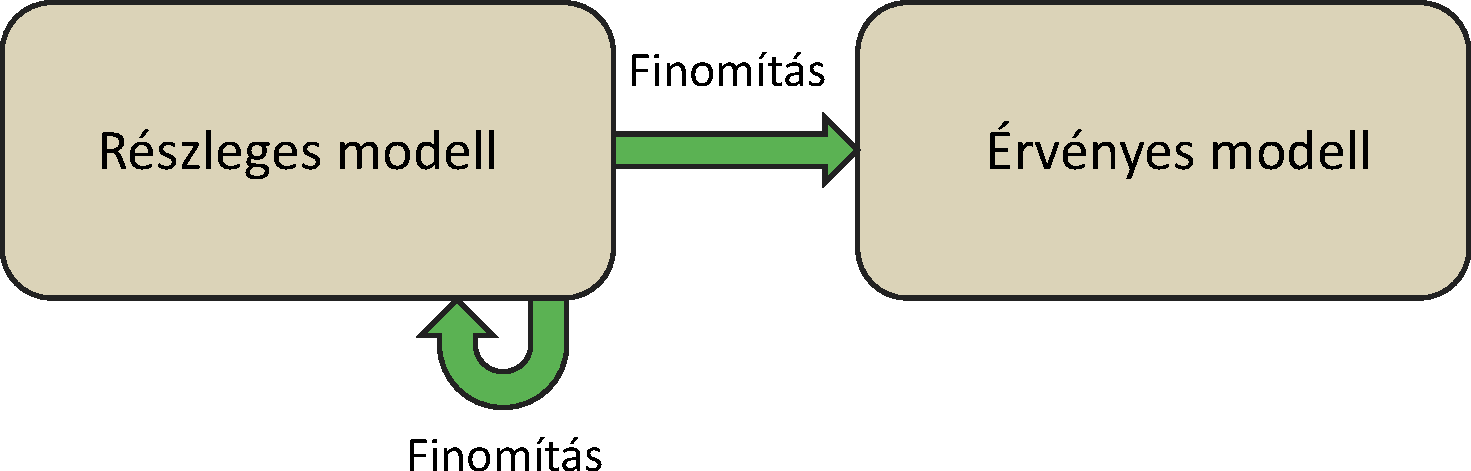
\includegraphics[width=120mm]{figures/finom.pdf}
	\caption{Finomítás menete} 
\end{figure}

\subsection{Szintaktika}
Részleges modellek esetén annotációkkal lehet megjelölni a modellt, illetve annak elemeit. Modellezés során 4 fajta részlegességet jelölhetünk meg. 
Annotációk
\subsection{Szemantika}
\subsubsection{May}

Annotációkkal láthatjuk el a modellt, az alapján, hogy egy modellelem biztosan benne lesz a végleges modellben, vagy pedig még bizonytalan a léte. ’M’ May exist(lehet, hogy benne lesz a végleges modellben), ’E’ Must exist(biztosan benne lesz a végleges modellben). A modell finomításával lépésről lépésre egyre kevesebb ’M’ lesz. ’M’ az vagy átvált ’E’ –re, vagy teljesen kikerül a modellből. Akkor tekinthető a modell véglegesnek, ha már nem szerepel benne ’M’-el megjelölt elem.
Tegyük fel, hogy nem tudjuk milyen járművet akarunk még modellezni a kezdeti fázisban. Ezért a kiindulási objektummodellben elláttuk May annotációkkal a járműnek az ajtó elemeit. Így finomítás során ezek az elemek később eltűnhetnek de akár meg is maradhatnak. Az a jármű aminek nincs ajtaja lehet akár egy motor, a két ajtós változat pedig egy autó.
\begin{figure}[htp]
	\centering
	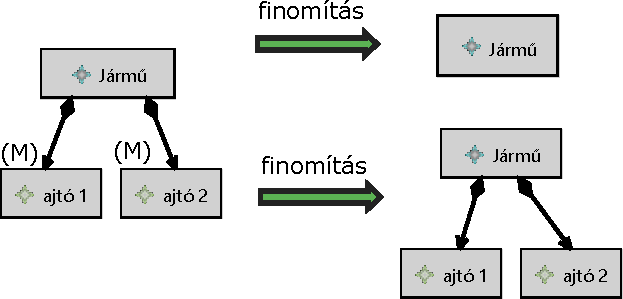
\includegraphics[height=50mm]{figures/may.pdf}
	\caption{May részlegesség feloldása} 
\end{figure}


\subsubsection{Abs}

Ennek is két különböző annotálási módja lehet: ’P’, Particular (egyedi elem) és ’S’, azaz Set (több elemet jelölhet). Particular az olyan elem, ami már biztosan benne lesz a végleges modellben, azonban a Set olyan elemet jelöl, ami lehet, hogy a végleges modellben több elemként fog megjelenni. Finomítások során az ’S’-el megjelölt
tagokat szétbontjuk több részre, de a végleges esetnél már csak particular, egyedi elemek szerepelhetnek.
Az alábbi ábra szerint első lépésben még nincs eldöntve, hogy az autónak egy vagy több motorja lesz. Ezt meg is jelöltük a megfelelő annotációval ('S'). Így a finomítás során lehetséges, hogy marad az egy motoros jármű, de lehet hogy szétbontjuk a motort és a járműbe rakunk egy benzinmotort és egy elektromos motort is.

\begin{figure}[htp]
	\centering
	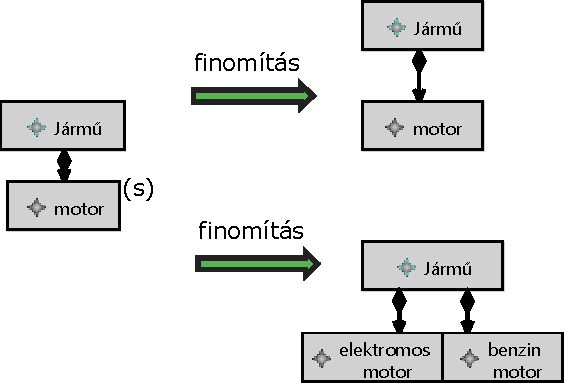
\includegraphics[height=50mm, keepaspectratio]{figures/abs.pdf}
	\caption{Abs részlegesség feloldása} 
\end{figure}

%\subsubsection{Var}

Kétféleképpen lehet annotálni az elemeket: ’C’ Constant (konstans elem) és ’V’ Variable (változó elem). Bizonyos értelemben az Abs fordítottjának lehet tekinteni. Felveszünk több elemet, ami lehet, hogy későbbiekben összeolvasztunk egy elemmé, tehát fenn áll a lehetősége annak, hogy két elem megegyezik. Amikor elkezdünk egy modellt, akkor nem biztos, hogy meg tudjuk mondani elemekről, hogy azok a későbbiekben azonosak-e vagy különbözőek. A végleges modellben már csak konstans elemek lehetnek.
Itt a példában látható, hogy a kezdeti állapotban még két külön kereke van a járműnek egyik kerekén kék dísztárcsa van a másik kereke pedig széles felnivel rendelkezik. Ezek meg lettek jelölve 'V' annotációval. Finomítás után ez megmaradhat ilyen különálló formában, de akár összeolvaszthatjuk ezt a két kereket és a végeredményben egy kerék marad, ami mind a kettő kerék tulajdonságát magában hordozza.

\begin{figure}[htp]
	\centering
	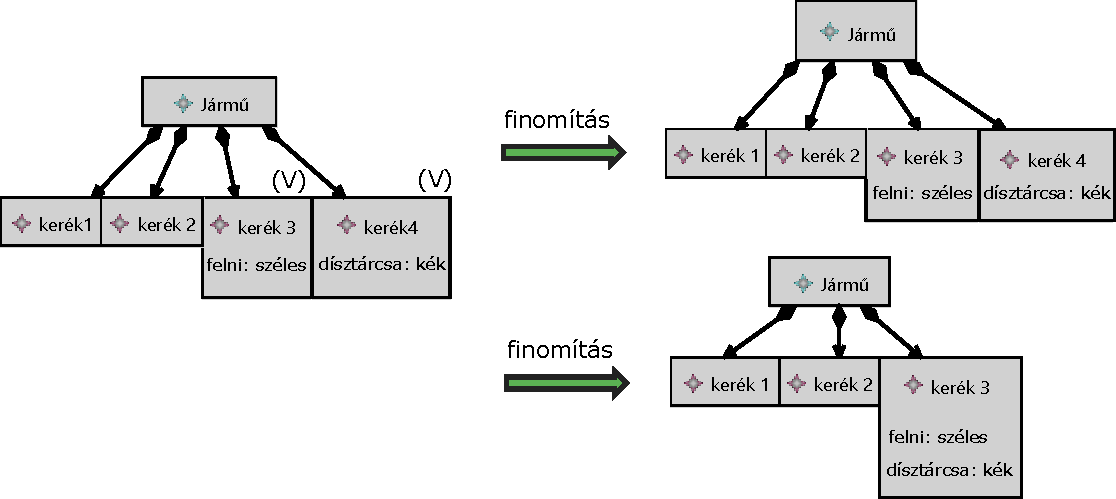
\includegraphics[height=50mm, keepaspectratio]{figures/var.pdf}
	\caption{Var részlegesség feloldása} 
\end{figure}

\subsubsection{OW}
Modellezés folyamán lehet megjelölni azt, hogy a modell már végleges e vagy sem. Ez a részlegesség nem a modell elemeire vonatkozik, hanem a teljes modellről árul el információt. 
